
\section{Results and discussions}
\label{results}

\begin{figure}[t]
	\centering
	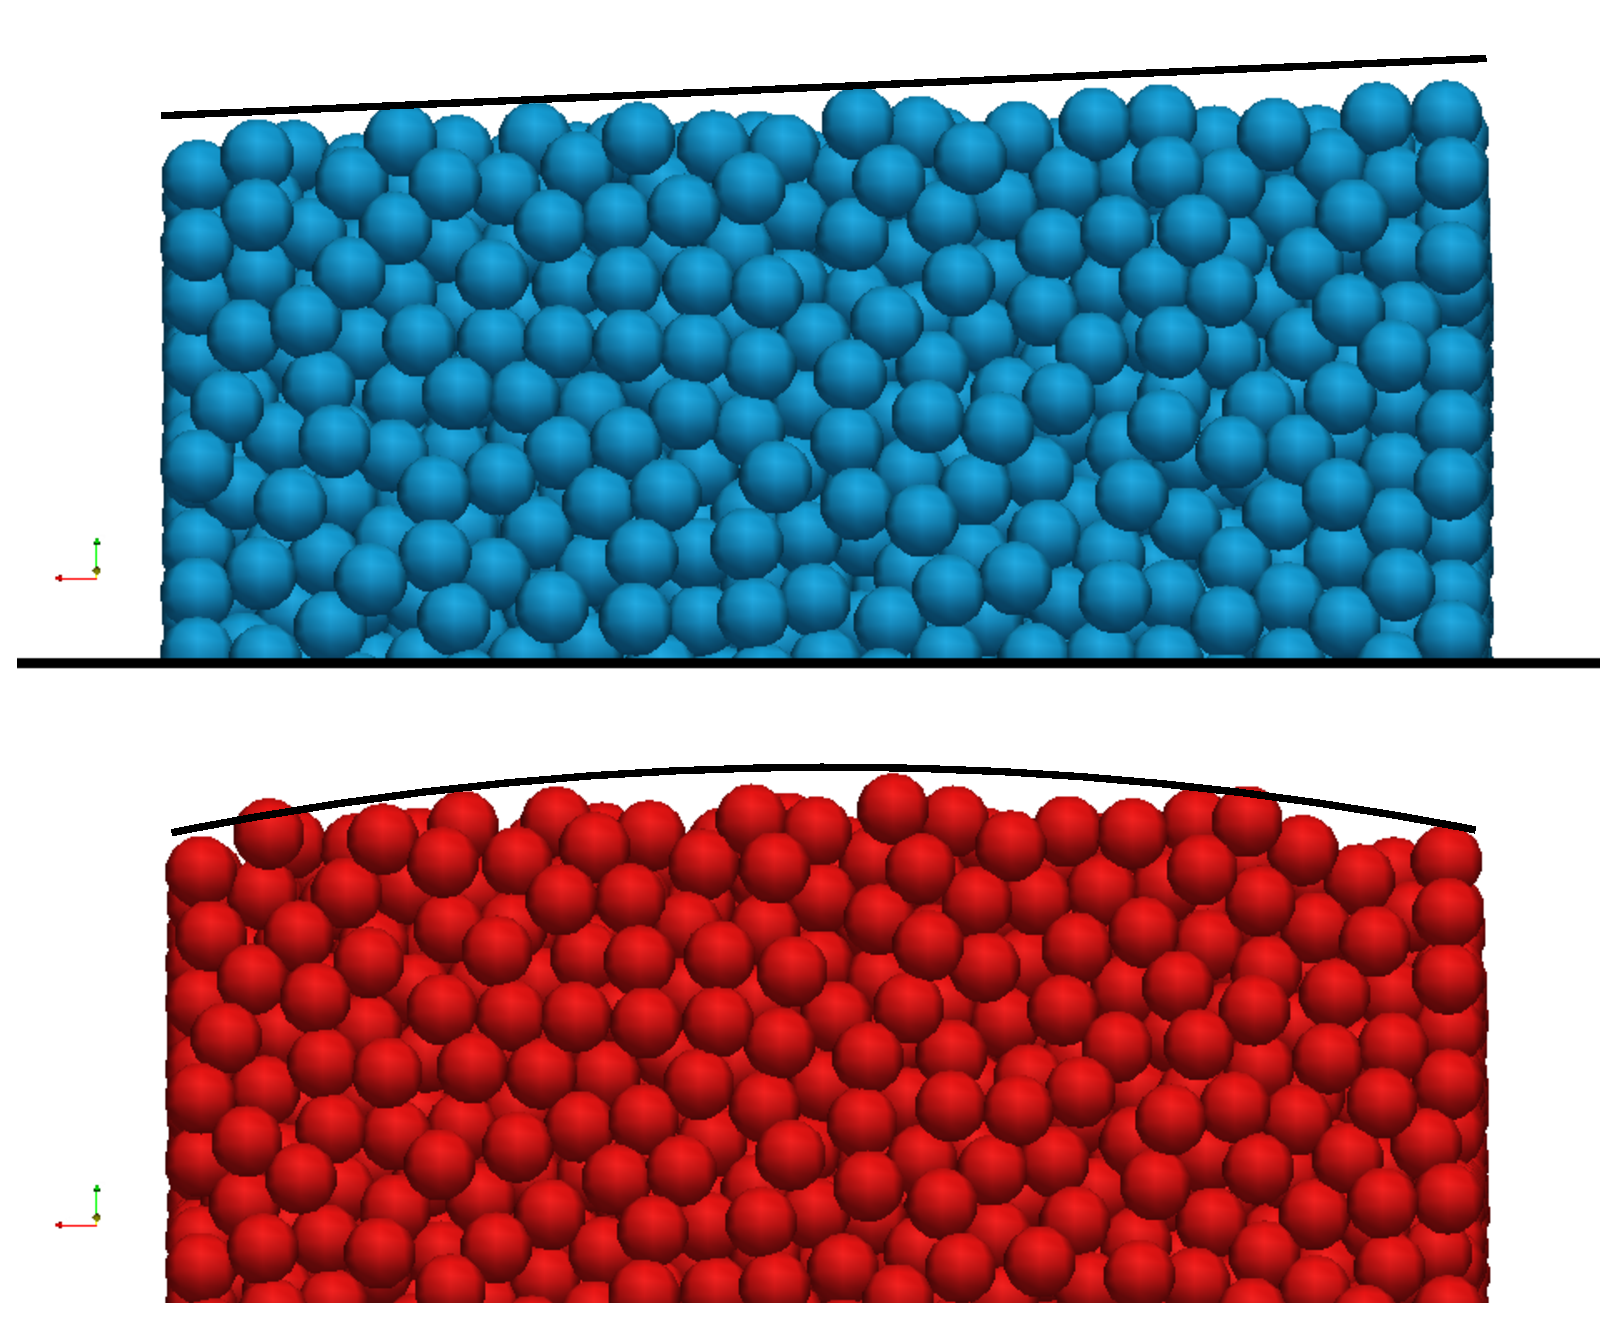
\includegraphics[width=0.4\textwidth]{chapters/figures/settlingStudy}
	\caption{Demonstrating the dynamic resettling from an example study done on location bias to pebble failure. The top image had the pebbles near the left wall biased to fail. The bottom image had a bias for the pebbles near both walls to fail. The lines are drawn as an aid to the eye.}
\label{fig:settlingStudy}
\end{figure}


The aim of this study was both to discover the impact of pebble failure on thermomechanical properties as well as determine the impact as a function of the number of failed pebbles. To satisfy the latter, we created beds with $\eta = 1\%$, $5\%$, $10\%$, and $15\%$ of pebbles failed. 

We first compare steady-state temperature profiles in the test beds against the one-dimensional theory of Eq.\ref{eq:continuum-heateqn}. To find the temperature profile in $x$, we create volumes of width $\Delta x$ that extend through the limits of the $y$- and $z$-directions. We then find the $n$ pebbles residing in the slices and take the mean value of their temperatures, $\langle T\rangle = \sum_{i}^n T_i / n$ of all pebble temperatures that have coordinates inside the slice. Below we will omit the notation $\langle T \rangle$ with the understanding that temperatures are volume-averages. Using the volume slices, we also find the average coordination number, $\langle Z \rangle = \sum_{i}^n Z_i / n$, normalized average contact force, $\langle F^* \rangle=\left[\langle F \rangle/\langle F_{bl} \rangle_\text{max}\right]^{1/3}$, and the normalized average temperature difference between pebbles in the slice, $\langle \Delta T_{ij} \rangle / (T_0 - T_s)_\text{bl}$; parameters which are discussed later.

When analytically solving Eq.~\ref{eq:thermoFirstLaw}, we introduce nondimensional temperature, $\theta_\text{1D} = (T -T_s)/(T_0-T_s)$, and spatial, $x^* = x/L$, variables and the solution becomes purely geometric; $\theta_\text{1D} = 1-x^{*2}$. We plot this theoretical solution against the temperature profiles coming from the steady-state DEM simulation in Fig.~\ref{fig:tempProfile}. We find that all our models had a nearly perfect match to a one-dimensional prediction, validating the calculation of effective thermal conductivity in this study. 

Another concern we had for pebble failure, was the phenomenon of `jamming' during resettling that would possibly leave pebbles isolated from their neighbors (apart from those they are resting upon). Such an isolated pebble would have no strong pathway for heat transfer and heat up much higher than that of its neighbors. Evidence of pebble isolation and `hot-spots' would be apparent in Fig.~\ref{fig:tempProfile} as localized deviations of data points from the quadratic profile. However, no deviations are seen in the data and we conclude that hot-spots will not be a concern in a packed bed.

\begin{figure}[t]
	\centering
	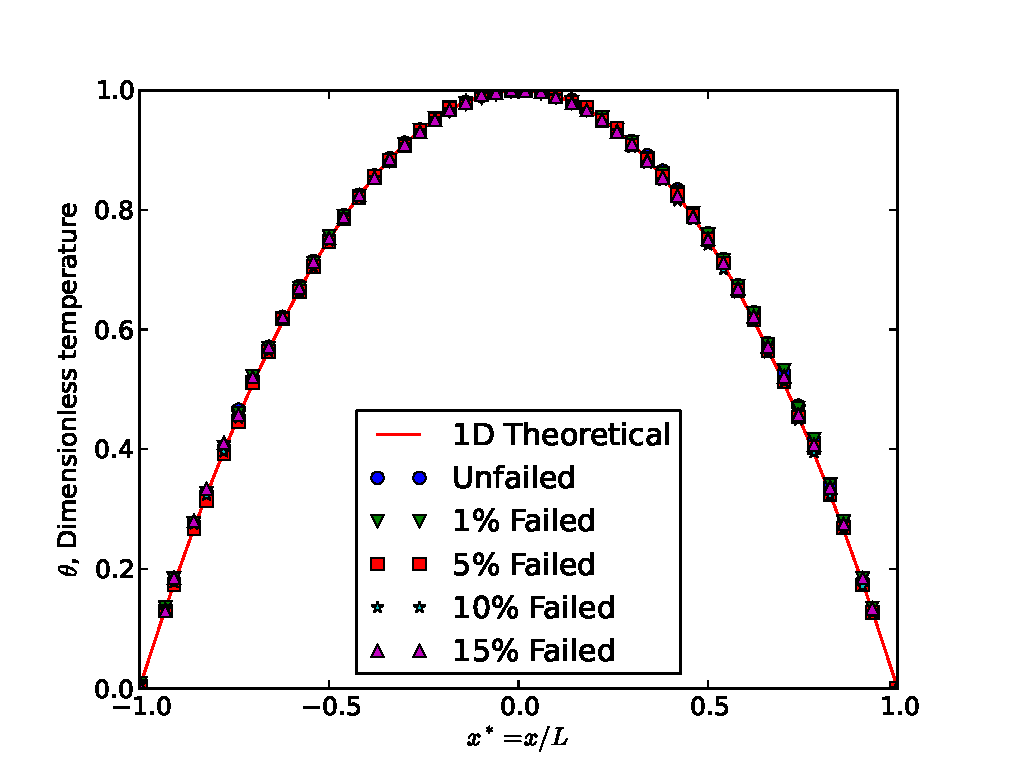
\includegraphics[width=0.5\textwidth]{chapters/figures/tempProfiles}
	\caption{The nondimensional temperature profiles for each test case follow the theoretical shape of a one-dimensional, constant $k$, continuum solution.}
\label{fig:tempProfile}
\end{figure}



\begin{figure}[t]
	\centering
	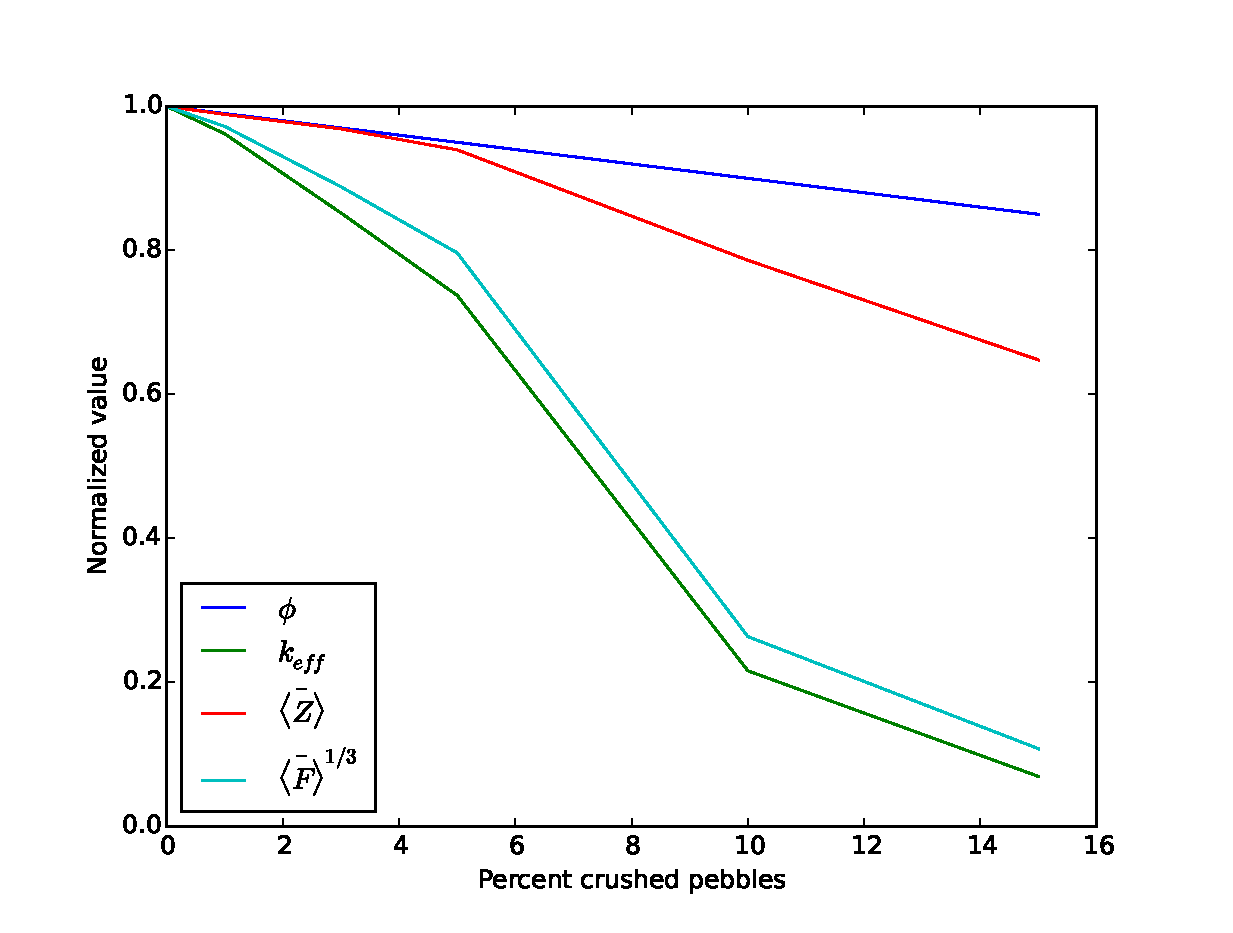
\includegraphics[width=0.5\textwidth]{chapters/figures/kEff_packingFraction}
	\caption{The normalized effective thermal conductivity (solid line) follows an exponential decay relationship with amount of failed pebbles. The normalized packing fraction (dashed line), compared to thermal conductivity, is relatively constant and is more closely fit to a linear reduction.}
\label{fig:packingFraction}
\end{figure}

\begin{figure}[t]
	\centering
	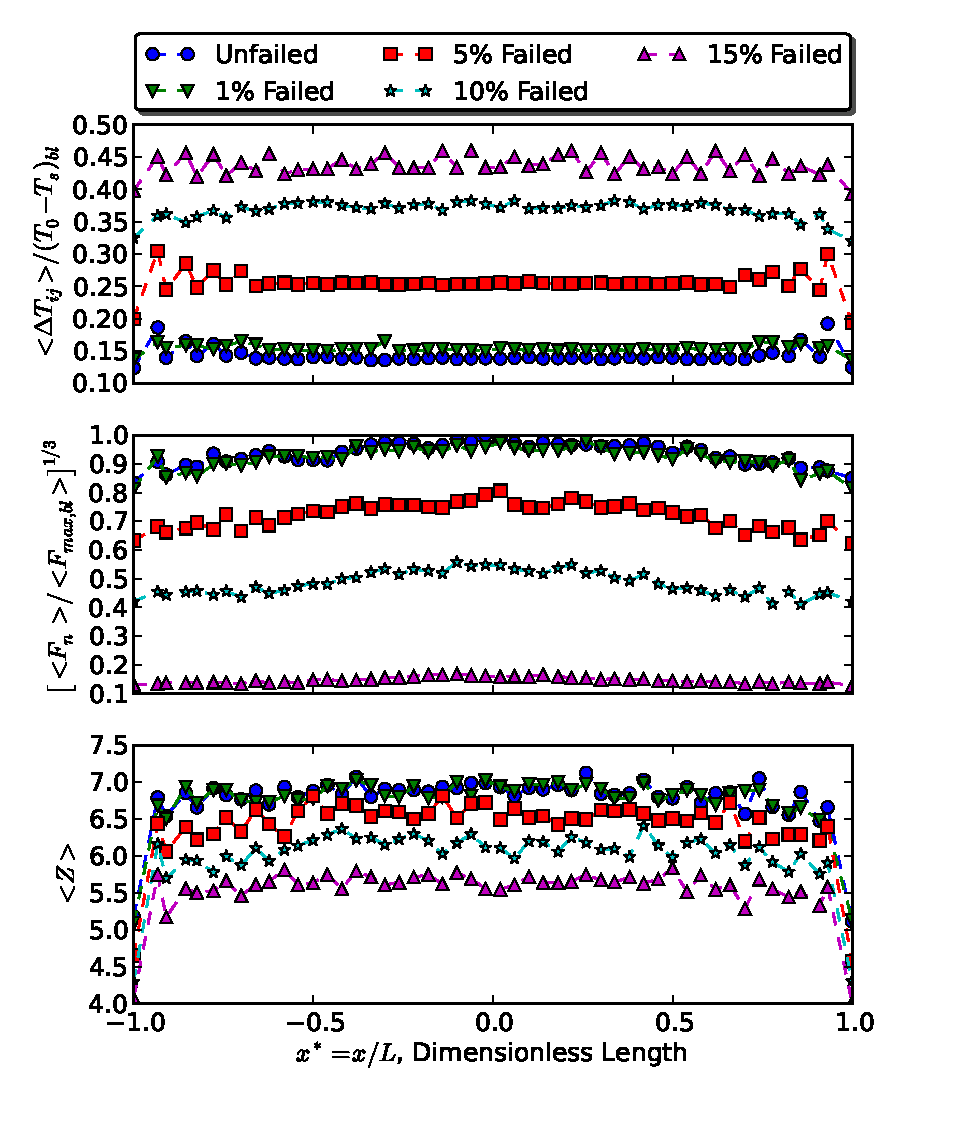
\includegraphics[width=0.5\textwidth]{chapters/figures/z_f_deltaT_subPlots}
	\caption{Average temperature differences between neighboring pebbles (top), contact forces (middle) and coordination numbers (bottom). The profiles of average coordination number and contact forces in the bed decrease in value with increasing pebble failure. Fewer and weaker contacts will reduce the possible paths of heat transfer from a pebble and this results in higher average temperatures between neighbors.}
\label{fig:coordProfiles}
\end{figure}


The effective thermal conductivity is found for all of our pebble beds, via Eq.~\ref{eq:etc}, then normalized against the conductivity of the baseline ensemble ($k_\text{eff}^* = k_\text{failed}/k_\text{bl}$). Figure~\ref{fig:packingFraction} shows the decreasing ETC with pebble failure. When $15\%$ of the pebbles are crushed in a pebble bed, the ETC has fallen all the way to only $k_\text{eff}^*=0.30$. This large reduction is especially important in light of the already poor thermal management of virgin pebble beds that, even in helium environments, have been experimentally measured at only approximately 1~W/m-K (see, { e.g.}, Refs.~\cite{Reimann:2002mi, Piazza2002}). In well-packed pebble beds, the ETC is generally related to the packing fraction. In Fig.~\ref{fig:packingFraction}, this relationship seems weak as the effective conductivity drops much more rapidly than does the packing fraction as the number of broken pebbles in the ensemble increases. To find the cause of decrease in conductivity and to make use of the information provided by DEM tools, we look to other parameters than the packing fraction.

From Eq.~\ref{eq:thermoFirstLaw}, in the steady-state, the energy input by nuclear heating must be balanced by the transport of heat out of a pebble into its neighbors. Inter-particle heat transfer is dictated by the number of neighboring contacts, temperature difference between pebbles, and the thermal conductance, $h_{ij}$ through the contact area. The thermal conductance is, itself, a function of material properties  (which are essentially constant here) and the force at the contact, going as $h_{ij} \propto F_n^{1/3}$. Thus, the net heat out is a function of the three variables as

\begin{align}
	Q_\text{net} =f( Z, F_n^{1/3}, \Delta T)
\end{align}



The variables affecting $Q_\text{net}$ are plotted in Fig.~\ref{fig:coordProfiles}. The average coordination number, shown in the bottom plot, decreases from a mid-line value of about 7.0 at the steady-state of the baseline case down to a mid-line value of 5.5 for the 15\% failed bed; a reduction of about 80\%. But this number doesn't compare with the large reduction in ETC which was $k_\text{eff}^*=0.30$. Clearly, there are fewer contacts in the pebble bed after failure but this alone does not account for the reduction in ETC.

Much more dramatic, seen in the center plot, is the reduction in average normal force seen by pebbles after many of the neighbors fail and are removed from the system. From the baseline down to the 15\% failed case, the contact forces are dramatically reduced to about $\langle F^* \rangle=0.1$.This reduction in force is joined by an increase in average neighbor temperatures which are 3 times higher for the bed with most failed pebbles when compared to the baseline. 

The results shown in Fig.~\ref{fig:coordProfiles} demonstrate that the heat transfer through a pebble bed is simultaneously a function of the coordination number and inter-particle contact forces -- which are both reduced as pebbles in the bed fail -- as well as the temperature difference between pebbles at steady state -- which increases as pebbles in the ensemble fail. Interestingly, when a pebble bed has lower overall inter-particle contact forces fewer particles would be expected to break. This would imply that pebble breakage is self-dampening; as pebbles begin to break the ensemble quickly relaxes and avoids future pebble failure. So while we induced failure up to $\eta = 15\%$, such large values may not occur in real beds. 

Another feature of Fig.~\ref{fig:coordProfiles} worth noting is the increase in averaged normal contact forces near the center of the bed relative to the walls. In the assumptions used to develop this simulation, we had noted the lack of localized force concentrations in a bed under an external mechanical load. However, in these results, owing to the nuclear heating temperature profile and thermal expansion of each pebble, there is a bias toward higher forces in the center of the bed. This result highlights the need for a model to predict failure initiation in place of the assumption of random pebble failure. 
%There are dramatic decreases near the walls for two reasons. The first being that contact of a pebble with a wall is not counted in the overall coordination number. The second is the forced ordering that pebbles experience near walls that is absent from the random packing in the bulk. Away from the walls, there is a clear decreasing trend in the coordination number as the pebble failure increases. From Eq.~\ref{eq:thermoFirstLaw}, the heat transfer from a pebble is a function of the number of neighbors with which the pebble is in contact. 

